\subsection{\textcolor{gray}{Detail of Design}}
The Smart Lock prototype consists of both hardware and software components, designed to provide secure, remote access control with user authentication and cloud connectivity.

\subsubsection{\textcolor{teal}{System Overview}}

Our system integrates a physical keypad-based lock with Wi-Fi-enabled remote access through a mobile application. Users can authenticate using a PIN or biometric authentication (fingerprint or facial recognition), and manage access remotely.

\begin{figure}[h]
    \centering
    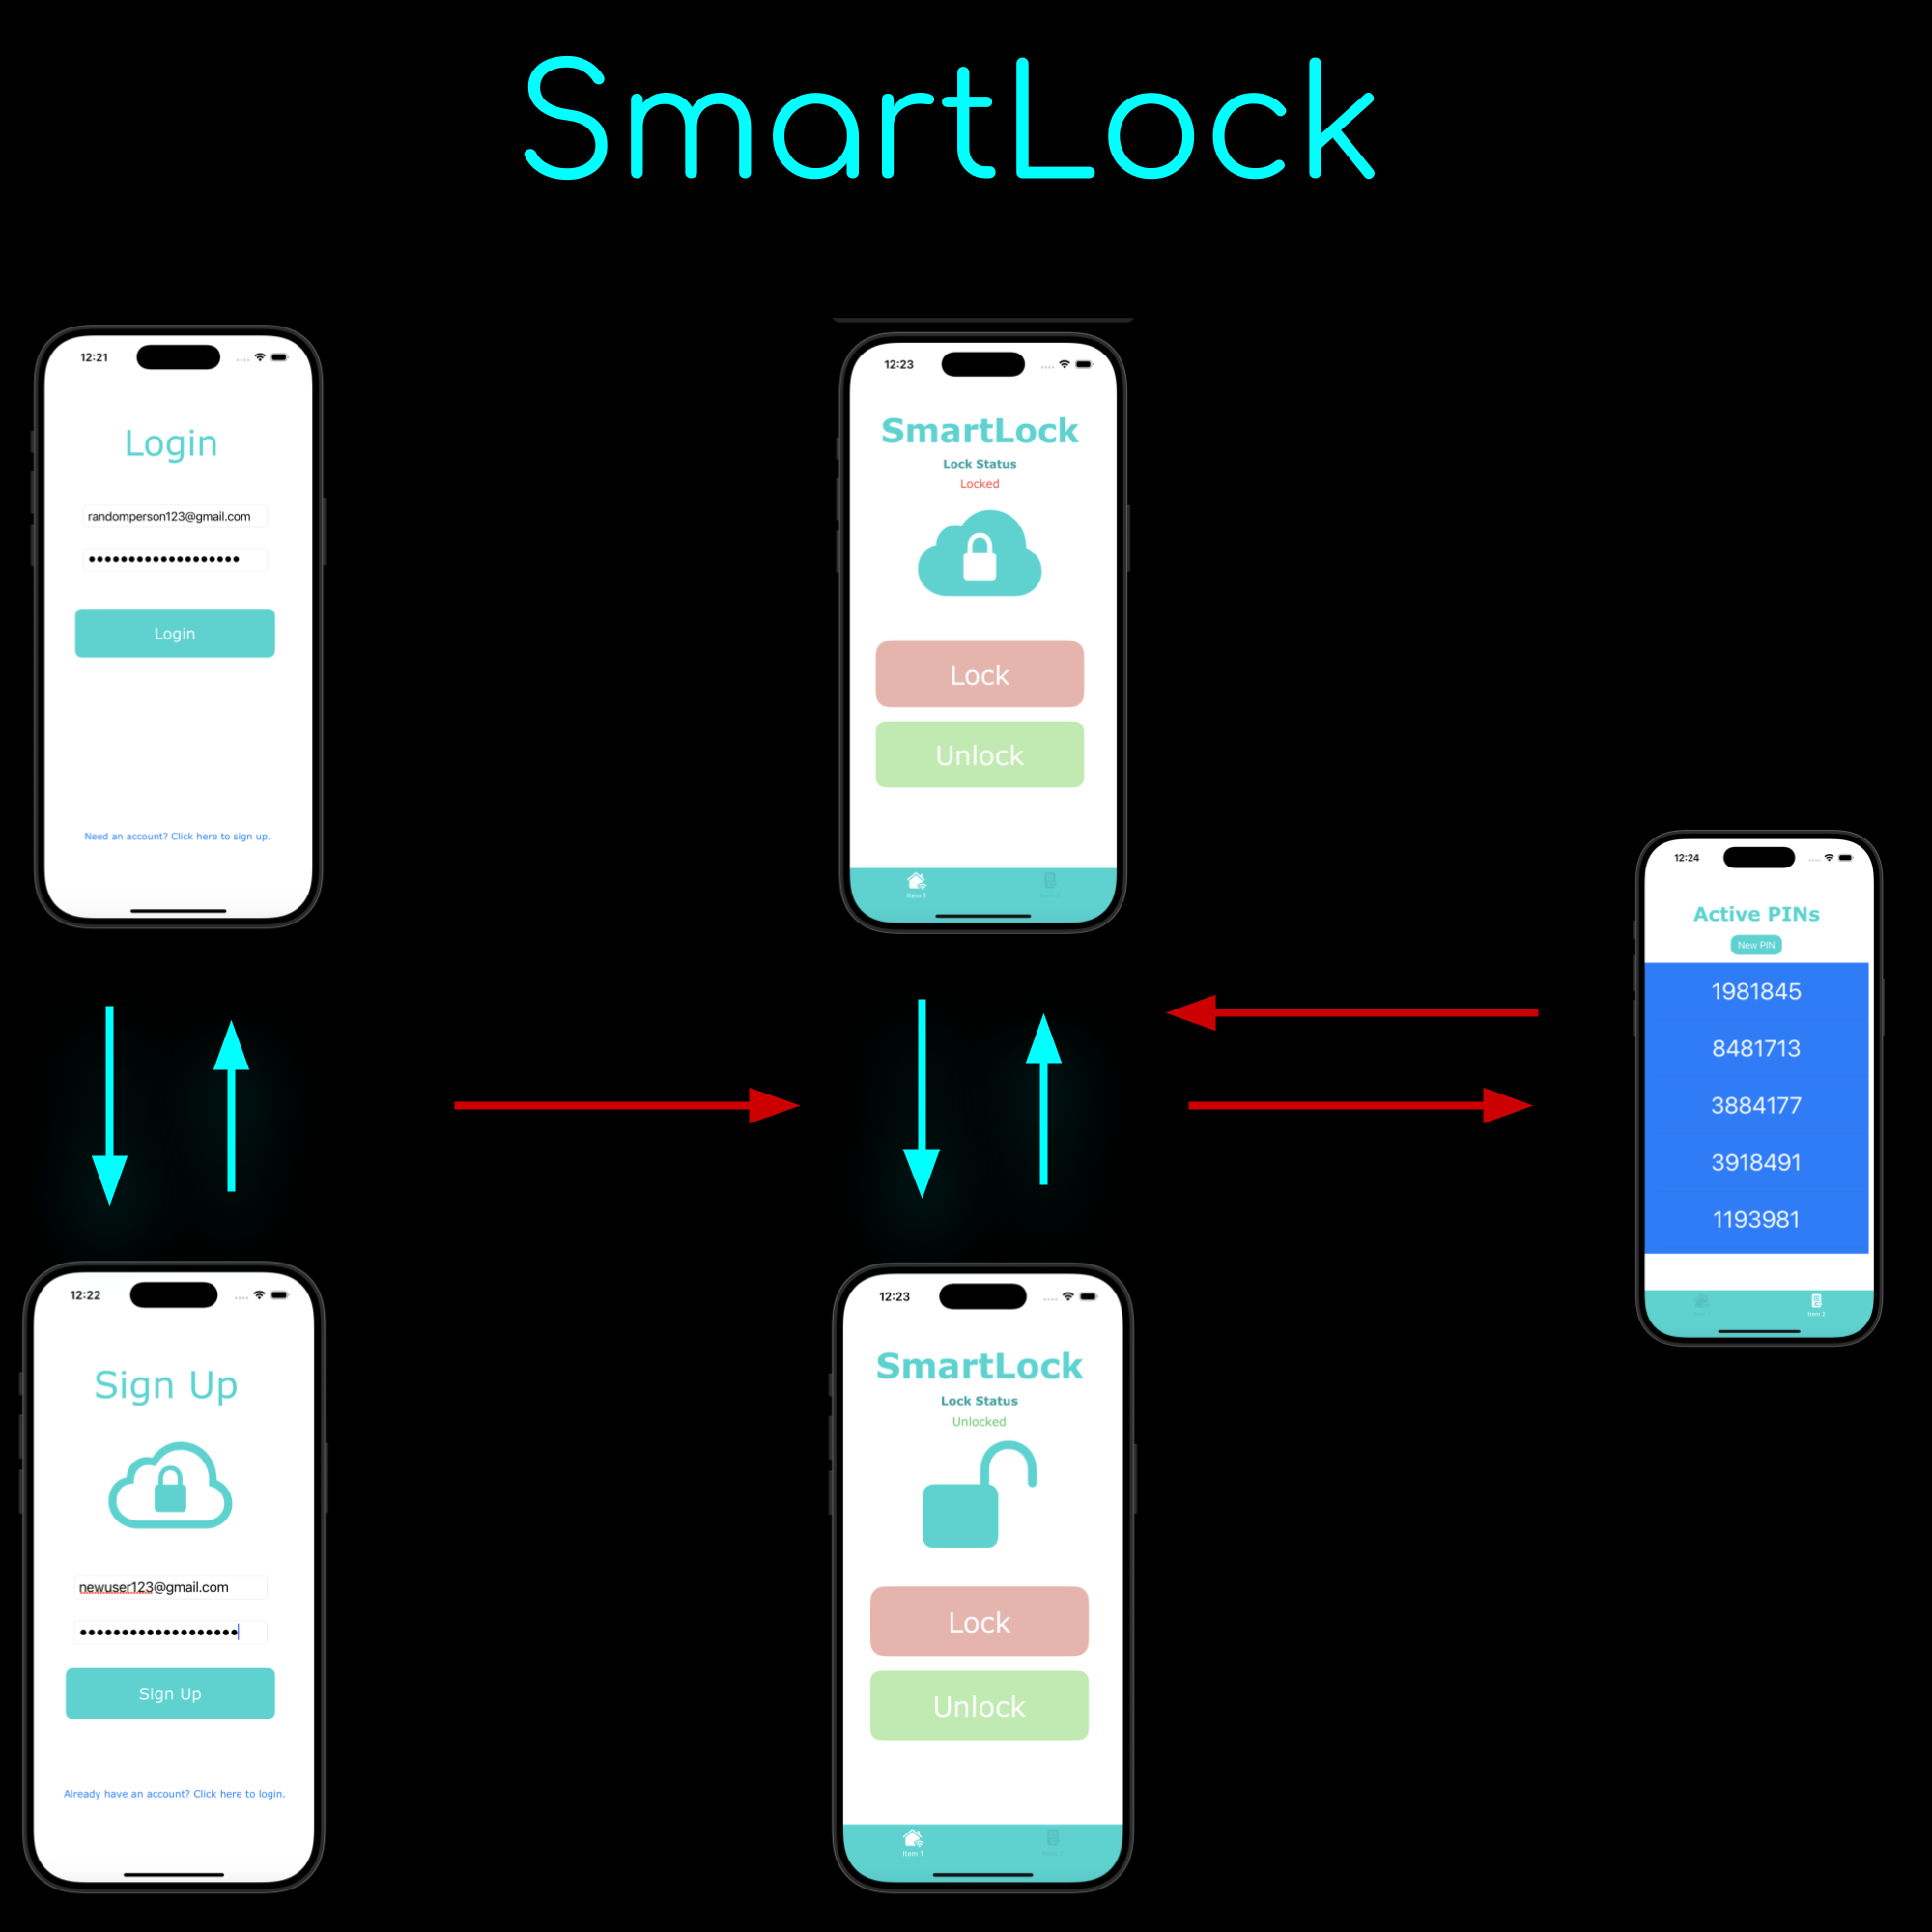
\includegraphics[width=0.65\textwidth]{flowsl.png}
    \caption{Mobile App Flowchart for Smart Lock System}
\end{figure}

\begin{itemize}
    \item Users log in or create an account to access the smart lock.
    \item The main control screen provides lock/unlock buttons.
    \item Users can view and manage active PIN codes for secure access.
    \item The system communicates with a cloud database (Firestore) for real-time authentication and remote control.
\end{itemize}

\subsubsection{\textcolor{teal}{Connectivity and Cloud Integration}}

The Smart Lock is cloud-connected, enabling users to manage access remotely via a mobile app. The system:
\begin{itemize}
    \item Authenticates PIN entries locally for quick access.
    \item Processes biometric authentication for increased security.
    \item Syncs PIN codes with Firebase, allowing updates in real-time.
    \item Sends lock/unlock status to the cloud, ensuring remote monitoring.
    \item Logs user access, creating an audit trail for security.
\end{itemize}

\subsubsection{\textcolor{teal}{Hardware Design}}

The Smart Lock hardware consists of a 3D printed casing, a keypad for PIN entry, a biometric scanner, a solenoid lock mechanism, and an ESP32-C3 microcontroller.

\begin{figure}[htbp]
    \centering
    \begin{subfigure}[b]{0.48\textwidth}
        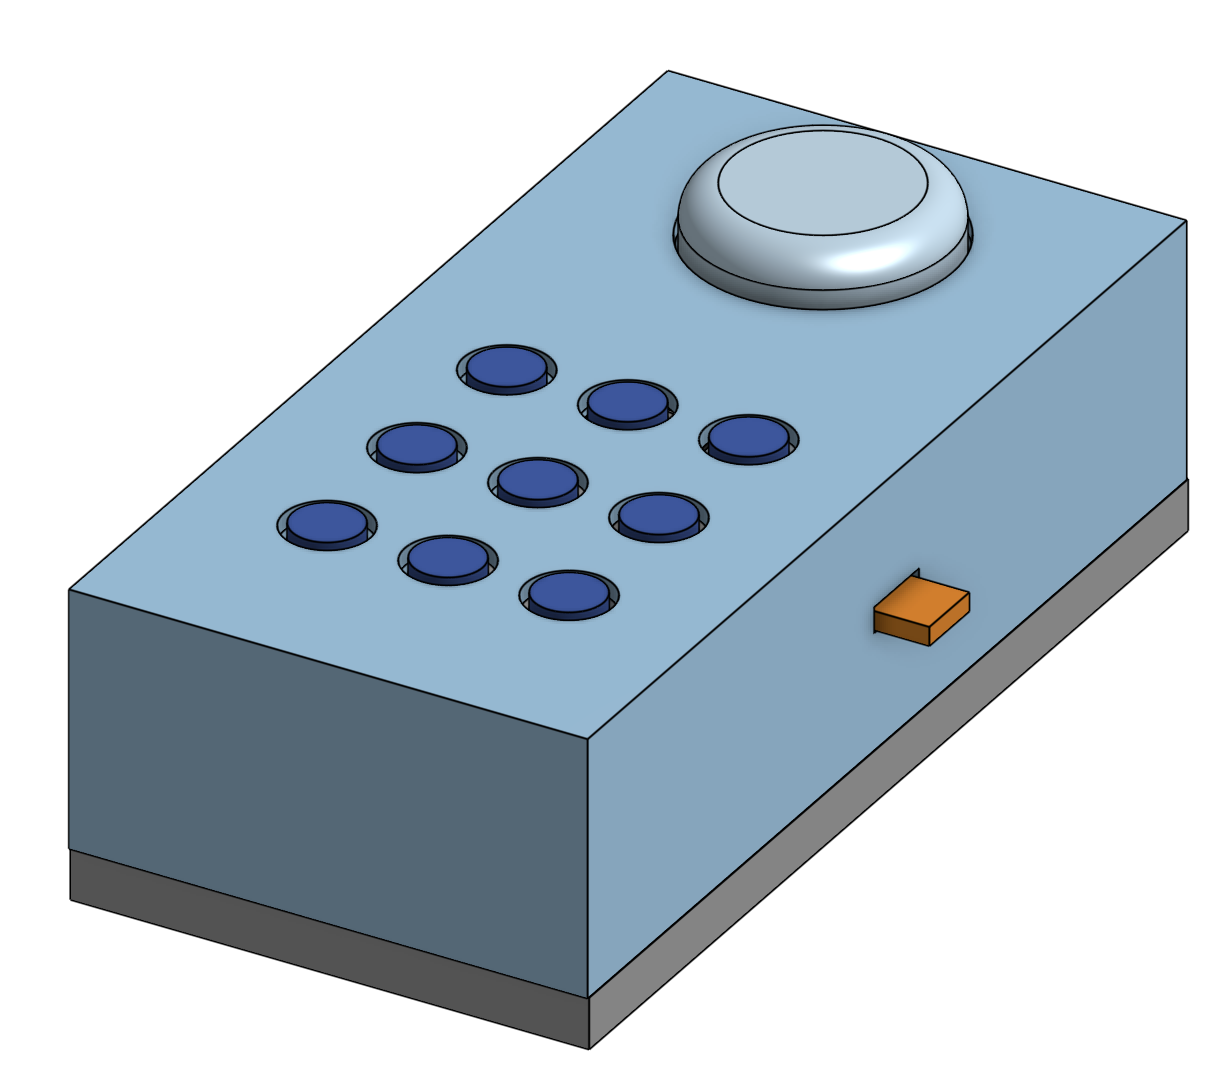
\includegraphics[width=\textwidth]{./isoView.png}
        \caption{Isometric View}
        \label{fig:isoView}
    \end{subfigure}
    \hfill
    \begin{subfigure}[b]{0.48\textwidth}
        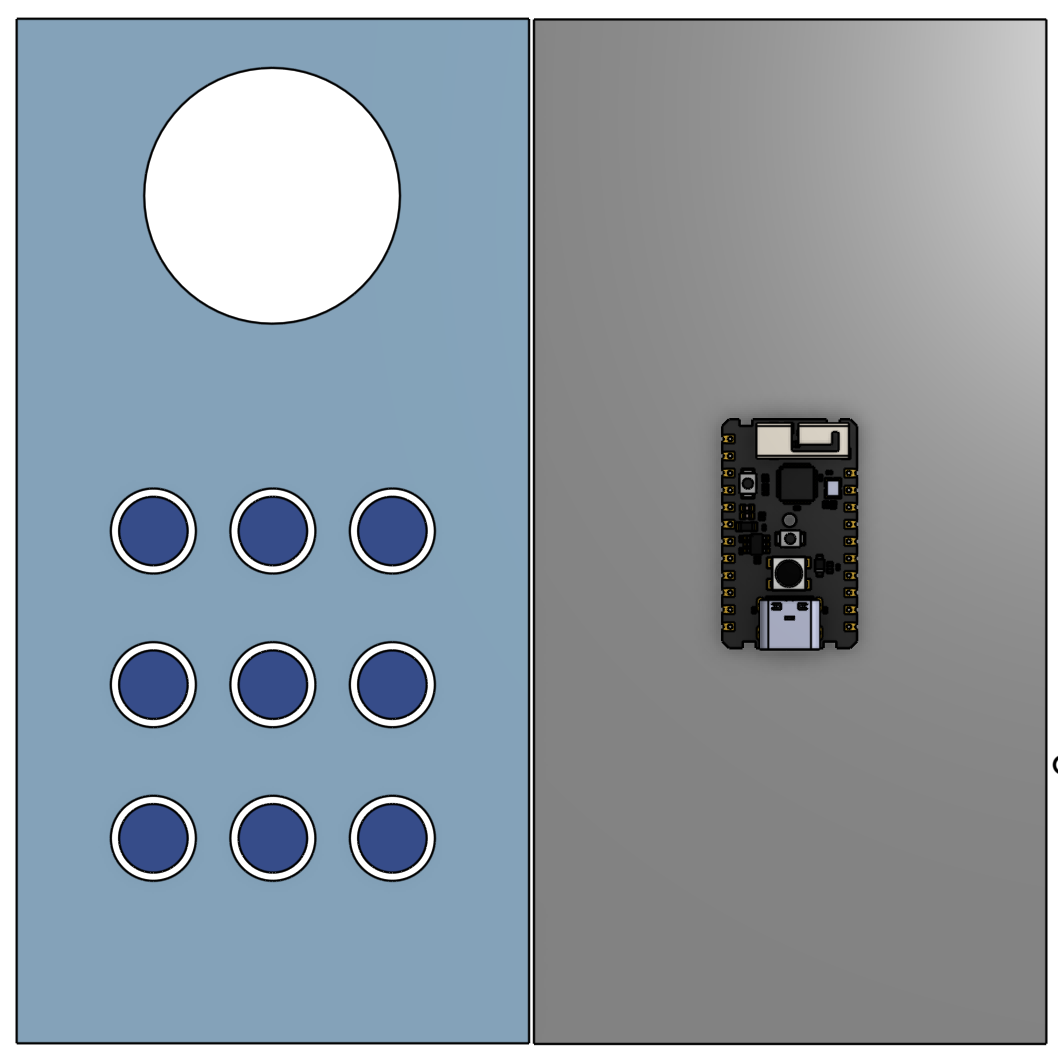
\includegraphics[width=\textwidth]{./topView.png}
        \caption{Top View}
        \label{fig:topView}
    \end{subfigure}
    \caption{First lock design}
\end{figure}

Here is the isometric view of the Smart Lock prototype. The top section will potentially include a biometric scanner, for fingerprint or facial recognition authentication, and a numeric keypad for PIN entry.\newline

\textbf{Key components:}
\begin{itemize}
    \item \textbf{Biometric Scanner:} Supports fingerprint or facial recognition for enhanced security
    \item \textbf{Numeric Keypad:} Users enter PIN codes as an alternative authentication method
    \item \textbf{Solenoid Lock:} Engages or disengages upon successful authentication
    \item \textbf{Microcontroller (ESP32-C3):} Handles user input, authentication, and connectivity
    \item \textbf{Rechargeable Battery:} Powers the system, ensuring reliability even in case of power outages
\end{itemize}

This design ensures compactness while maintaining modular repairability, allowing components to be easily accessed or replaced.


\subsubsection{\textcolor{teal}{Life Cycle Assessment (LCA)}}

The life cycle of the Smart Lock was analyzed to ensure sustainability and environmental responsibility. Key aspects include: \newline

\textbf{Eco-Friendly Manufacturing}
\begin{itemize}
    \item Uses locally sourced materials to minimize transportation emissions
    \item Modular design allows for easy repair and component replacement, reducing e-waste
    \item Prioritizes recyclable materials in construction
\end{itemize}

\textbf{Energy Efficiency}
\begin{itemize}
    \item Operates on a rechargeable lithium battery to extend lifespan
    \item Supports an optional solar charging module to reduce reliance on disposable batteries
\end{itemize}

\textbf{Smarter Chemistry}
\begin{itemize}
    \item Lead-free soldering eliminates hazardous materials.
    \item Arsenic- and mercury-free components ensure environmental safety.
    \item PVC-free wiring minimizes harmful plastic waste.
\end{itemize}

\textbf{End of Life Considerations}
\begin{itemize}
    \item Designed for easy disassembly, allowing parts to be recovered for recycling.
    \item Encourages users to recycle old locks through e-waste partnerships.
\end{itemize}

\textbf{Commitment to Sustainability}
\begin{itemize}
    \item Uses stainless steel casing with the option for recycled metal integration.
    \item Packaging minimizes non-recyclable plastics, favoring biodegradable materials
\end{itemize}

\begin{figure}[h]
    \centering
    \includegraphics[width=0.8\textwidth]{LifeCycle.png}
    \caption{Life Cycle Assessment of the Smart Lock}
    \label{fig:lifecycle}
\end{figure}

\noindent By integrating secure hardware, cloud-based software, and sustainable practices, the Smart Lock aims to offer a modern, environmentally responsible solution to traditional key-based access control.